\documentclass[a4paper,twocolumn,10pt]{article}
\usepackage[spanish]{babel}
\usepackage[T1]{fontenc}
\usepackage[utf8]{inputenc}
\spanishdecimal{.}
\usepackage{lmodern}
\usepackage[a4paper]{geometry}
\usepackage{graphicx}
\usepackage{flushend}
\usepackage{wallpaper}
\usepackage{amsmath}
\usepackage{float}
\usepackage{colortbl}

\begin{document}

\title{Determinación de Líneas de Emisión de Distintos Elementos Mediante el Uso de un Espectrofotómetro. }
\author{ \\Aldo Aliaga, Benjamín Yapur, Fabian Trigo \\ \textit{Departamento de Física y Astronomía, Universidad de Valparaiso}}
\twocolumn[
  \begin{@twocolumnfalse}
    \maketitle
    \begin{abstract}
    Este experimento tiene como objetivo la determinación de los peaks en el espectro de frecuencias de cada elemento (líneas de emisión), para lograr esto, con el uso de un espectrofotómetro y una fuente de luz correspondiente a cada elemento, medimos y comparamos los peaks obtenidos experimentalmente con la teoría, obteniendo así una mediana del error de $1.1 \times 10^{-8}$, predicha por la incertidumbre calculada en nuestro analisis.
    \end{abstract}
  \end{@twocolumnfalse}\bigskip]

\vspace{2cm}

\section{Introducción}
Todo elemento químico emite en longitudes de onda características cuando son excitados por una descarga eléctrica. Mediante el aumento de energía de sus electrones y la emisión de fotones al volver a su estado original. 

En este experimento se hace uso de un espectrofotómetro, el cual mediante una rejilla difractante separa la luz en ángulos $\theta$ de acuerdo a su longitud de onda. La ecuación que expresa la difracción máxima (punto en donde dos crestas o dos canales se juntan) es:

\begin{equation}
    d\sin{\theta}=n\lambda
\end{equation}

Donde $d$ es la distancia entre las rendijas de la rejilla y n es el orden de difracción.

\section{Montaje Experimental}
\subsection{Herramientas}
\begin{itemize} 
\item Espectrofotómetro
\item Interfaz Pasco®
\item Lampara con distintas ampolletas con elemenos a analizar
\item Lona para cubrir luz externa
\item Colimador
\item Lentes
\item Grilla de difracción
\end{itemize}

\begin{figure}[H]
    \centering
    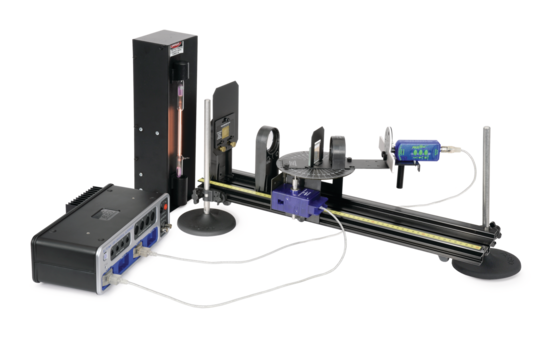
\includegraphics{md_sl8Mw4f2V8G6.png}
    \caption{Montaje de espectofotómetro.}
    \label{fig:my_label}
\end{figure}

\subsection{Procedimiento experimental}
Primero se cubre el espectrofotómetro con telas negras para evitar contaminación externa de luz sobre el sensor, se ha de construir con el colimador junto a la lampara para que entonces pase por los lentes y la grilla de difracción.

Luego se enciende la lámpara del elemento o molécula seleccionado, se procede a mover el plato graduado con el sensor de movimiento giratorio para que cada línea llegue al sensor de luz. El sensor de luz registra la intensidad luminica, especialmente de los peaks donde se hallan las líneas de luz difractadas, las cuales coinciden con las lineas de emision de los elementos.

Los datos recopilados de intensidad y ángulos son recopilados por la interfaz Pasco® para luego ser analizados.

Si realizamos varios barridos para un lámpara de un elemento se observa:
\begin{figure}[H]
    \centering
    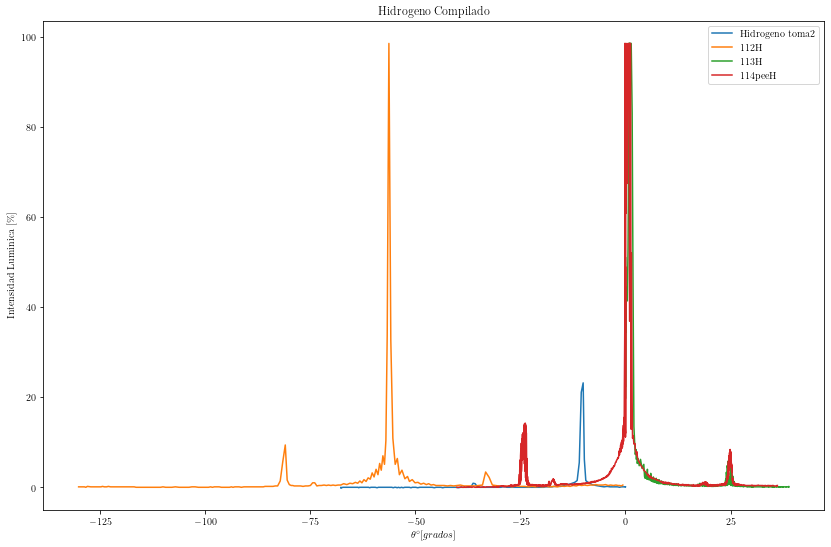
\includegraphics[width=0.5\textwidth]{Plots/HidrogenoCompilado.png}
    \caption{Multiples Tomas del Hidrogeno, se selecciono la curva roja}
    \label{fig:compund_hydrogen}
\end{figure}

Estos entonces son registrados por el software propio de pasco y analizados con una libreria de programación como matplotlib.


\section{Análisis}
Al realizar multiples barridos se debe tener en cuenta el orden de los datos, utilizando la libreria Pandas de Python junto a Numpy se consigue ordenar para conseguir una distribución continua, se puede observar en las siguientes figuras:

\begin{figure}[H]
    \centering
    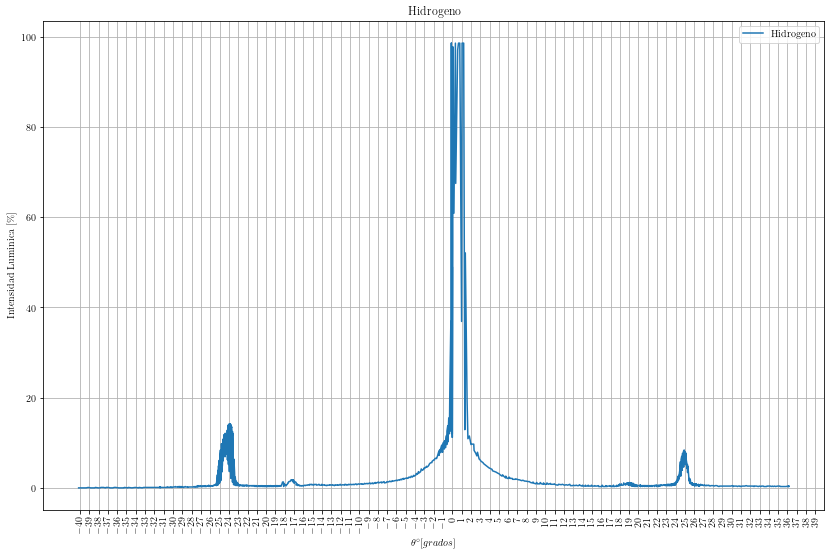
\includegraphics[width=0.5\textwidth]{Plots/Hidrogeno.png}
    \caption{Hidrógeno}
    \label{fig:my_label}
\end{figure}

\begin{figure}[H]
    \centering
    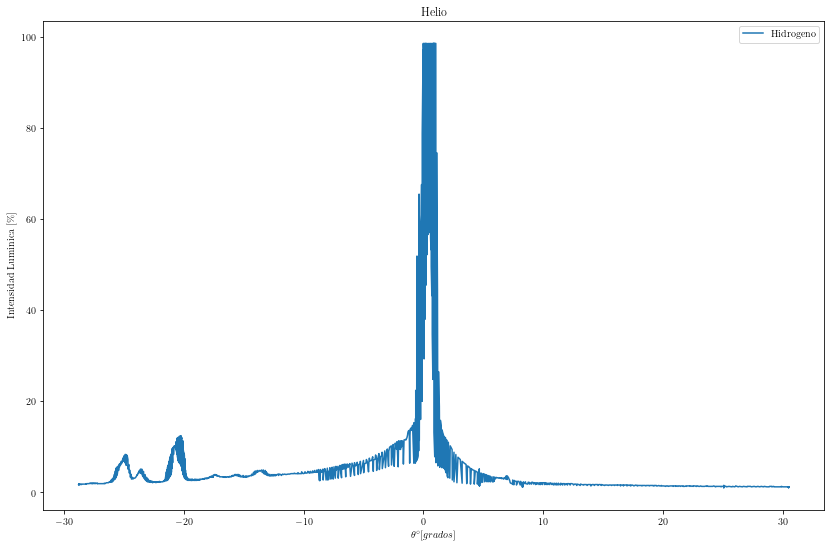
\includegraphics[width=0.5\textwidth]{Plots/Helio.png}
    \caption{Hidrógeno}
    \label{fig:my_label}
\end{figure}

\begin{figure}[H]
    \centering
    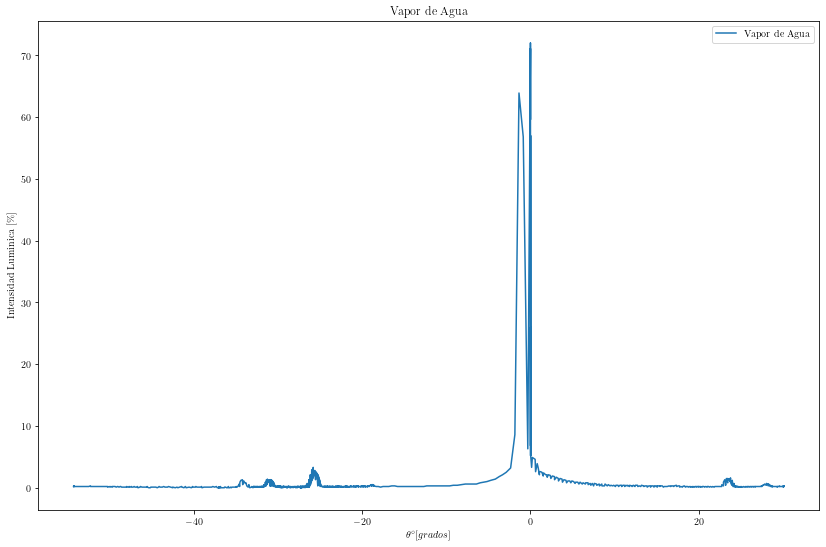
\includegraphics[width=0.5\textwidth]{Plots/Vapor de Awa.png}
    \caption{Vapor de Agua}
    \label{fig:my_label}
\end{figure}

\begin{figure}[H]
    \centering
    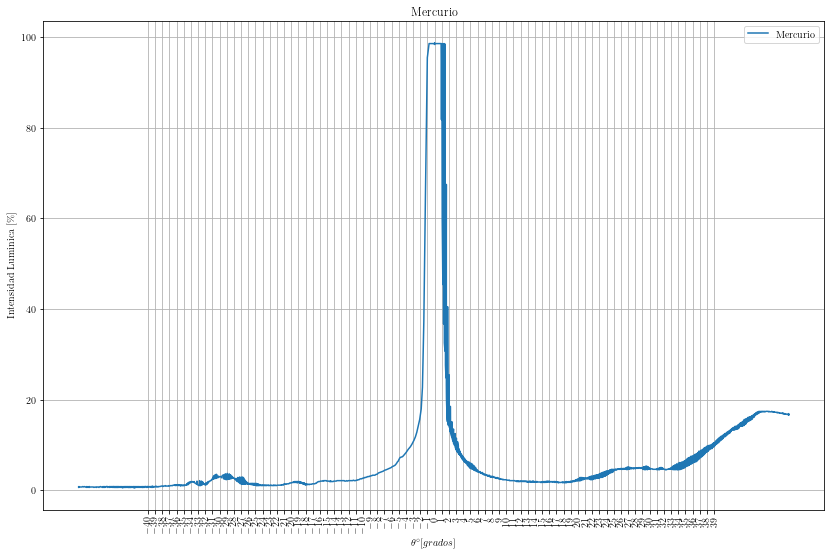
\includegraphics[width=0.5\textwidth]{Plots/Mercurio.png}
    \caption{Mercurio}
    \label{fig:my_label}
\end{figure}
\bigskip
\bigskip
Para analizar los peaks, funciones computarizadas entregaban poca informacion debido a la cantidad de ruido. Entregando los maximos locales necesarios pero con varios otros datos inservibles, volviendolo así un método poco efectivo. 
En su lugar se optó por incrementar los ticks en el grafico y analizarlo de forma visual, entregando una incertidumbre al ángulo de medio grado, la cual ya se encuentra considerada dentro de la incertidumbre del instrumento; un solo grafico con este método aplicado se puede observar en la Figura 8 (Analisis de $\lambda$ para Vapor de Agua)

%% --- grafico de analisis
\begin{figure}[H]
    \centering
    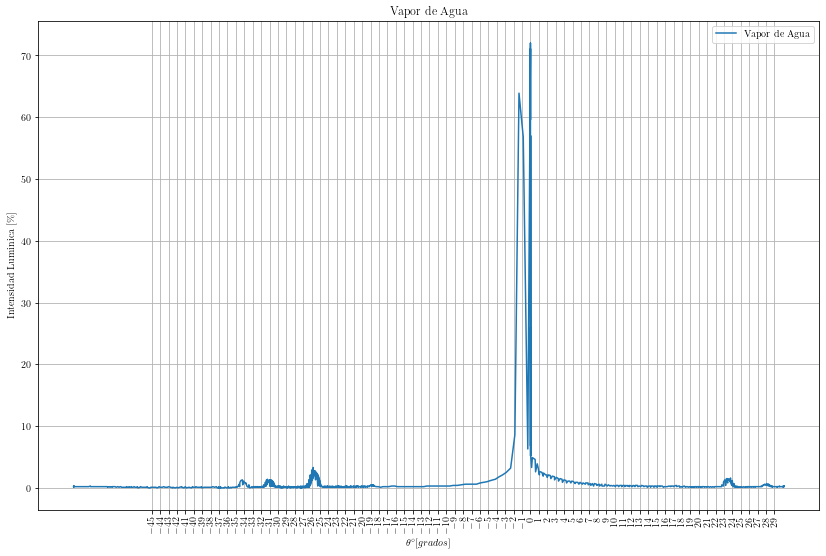
\includegraphics[width=0.5\textwidth]{Plot Analisis/Vapor de Agua.png}
    \caption{Análisis de $\lambda$ para Vapor de Agua}
    \label{fig:my_label}
\end{figure}
%----

Entonces se obtuvo los siguientes peaks en cada elemento:


\begin{table}[H]
\centering
\caption{Tabla 1, Medidas Numericas de los Máximos Locales con su Ángulo en Grados, Listados en Variables Categoricas de "diminuto", "significativo", "visible", "peak"}
\begin{tabular}{lllll}
{\cellcolor{cyan}}Argon         & {\cellcolor{cyan}}$\theta$ &  & {\cellcolor{cyan}}Helio    & {\cellcolor{cyan}}$\theta$  \\
diminuto                     & 18                                          &  & peak                       & 0                                            \\
significativo           & 30.5                                        &  & visible                    & 13.5                                         \\
significativo                   & 32                                          &  & diminuto                   & 15.5                                         \\
visible                         & 38                                          &  & diminuto                   & 17.5                                         \\
peak                            & 2                                           &  & significativo              & 20.5                                         \\
peak                            & -2                                          &  & significativo              & 23.5                                         \\
                                &                                             &  & significativo              & 25                                           \\
                                &                                             &  &                            &                                              \\
{\cellcolor{cyan}}Hidrógeno     & {\cellcolor{cyan}}$\theta$ &  &                            &                                              \\
peak                            & 0                                           &  &                            &                                              \\
visible                         & 17.5                                        &  &                            &                                              \\
significativo                   & 24                                          &  & {\cellcolor{cyan}}Mercurio & {\cellcolor{cyan}}$\theta$  \\
                                &                                             &  & peak                       & 0                                            \\
                                &                                             &  & visible                    & -4                                           \\
{\cellcolor{cyan}}Vapor de Agua & {\cellcolor{cyan}}$\theta$ &  & diminuto                   & 15.5                                         \\
peak                            & 0                                           &  & diminuto                   & 19.5                                         \\
significativo                   & 25                                          &  & significativo              & 27                                           \\
diminuto                        & 19                                          &  & significativo              & 29                                           \\
significativo                   & 31                                          &  & significativo              & 30.5                                         \\
significativo                   & 34                                          &  & visible                    & 34                                          
\end{tabular}
\end{table}


utilizando la relación entre la grilla de difracción y el ángulo, se puede calcular la longitud de onda asociada a cada uno de estos picos o peaks.

$$
d \sin \theta = n \lambda
$$

Para los cálculos se usa $d=1.67 \times 10^{-6} [m]$ la cual es la separación entre las distintas rendijas de esta grilla, al usar dos decimales tendremos una incertidumbre asociada, pero es un efecto minimo comparado a la incertidumbre del angulo $\theta$.

El $n$ es el orden y debido al setup los primeros ordenes ($n=1$) son con los que se realizan los calculos, sin embargo se incluye en la tabla el caso de asumir $n=2$, para considerar su uso

\begin{table}[H]
\centering
\caption{Tabla 2, Máximos Locales en la Distribución para el Cálculo de la Longitud de Onda}
\begin{tabular}{lll}
\rowcolor[rgb]{0,1,0.914} Peaks         & n=1       & n=2       \\
\rowcolor[rgb]{0,1,0.914} Argon         &           &           \\
18                                      & 5.15E-07  & 2.58E-07  \\
30.5                                    & 8.46E-07  & 4.23E-07  \\
32                                      & 8.83E-07  & 4.42E-07  \\
38                                      & 1.03E-06  & 5.13E-07  \\
2                                       & 5.82E-08  &           \\
-2                                      & -5.82E-08 &           \\
                                        &           &           \\
\rowcolor[rgb]{0,1,0.914} Helio         &           &           \\
0                                       & 0.00E+00  &           \\
13.5                                    & 3.89E-07  & 1.95E-07  \\
15.5                                    & 4.45E-07  & 2.23E-07  \\
17.5                                    & 5.01E-07  & 2.51E-07  \\
20.5                                    & 5.84E-07  & 2.92E-07  \\
23.5                                    & 6.65E-07  & 3.32E-07  \\
25                                      & 7.04E-07  & 3.52E-07  \\
                                        &           &           \\
\rowcolor[rgb]{0,1,0.914} Hidrógeno     &           &           \\
0                                       & 0.00E+00  &           \\
17.5                                    & 5.01E-07  & 2.51E-07  \\
24                                      & 6.78E-07  & 3.39E-07  \\
                                        &           &           \\
\rowcolor[rgb]{0,1,0.914} Mercurio      &           &           \\
0                                       & 0.00E+00  &           \\
-4                                      & -1.16E-07 &           \\
15.5                                    & 4.45E-07  & 2.23E-07  \\
19.5                                    & 5.56E-07  & 2.78E-07  \\
27                                      & 7.57E-07  & 3.78E-07  \\
29                                      & 8.08E-07  & 4.04E-07  \\
30.5                                    & 8.46E-07  & 4.23E-07  \\
34                                      & 9.32E-07  & 4.66E-07  \\
                                        &           &           \\
\rowcolor[rgb]{0,1,0.914} Vapor de Agua &           &           \\
0                                       & 0.00E+00  &           \\
25                                      & 7.04E-07  & 3.52E-07  \\
19                                      & 5.43E-07  & 2.71E-07  \\
31                                      & 8.58E-07  & 4.29E-07  \\
34                                      & 9.32E-07  & 4.66E-07 
\end{tabular}
\end{table}

En la tabla los valores negativos se utilizan para representar que es un peak máximo que cubre ángulos hasta ese punto, pudiendo representar difracciones de primer orden ($n=1$)

Teniendo en cuenta las siguientes incertidumbres a las medidas, $\Delta d = 0.01 \times 10^{-6}=10^{-8}$, se propaga errores de lambda como una función

$$(\Delta \lambda)^2 \leq (\frac{\partial \lambda}{\partial \theta} \Delta \theta)^2|_z + (\frac{\partial \lambda}{\partial d} \Delta d)^2|_{z'}$$

donde $z,z'$ maximizan las funciones dentro del rango de las variables, entregando así la incertidumbre máxima, dejándolo de la forma
$
\Delta \lambda \leq \sqrt{
    (d \Delta \theta)^2 + (\Delta d)^2
}
$.
La incertidumbre de las longitudes de onda $\Delta \lambda \leq 1.8 \times 10^{-8}$ aproximandola hacia un solo dígito
$$
\Delta \lambda \leq 2 \times 10^{-8}
$$

Se ha de notar que desconocemos el orden n de esta relación angulo longitud de onda, sin embargo, teniendo en cuenta la incertidumbre podemos continuar la tabla $n=1$ tomando el primer valor, entonces situados en la tabla $n=2$ buscar esta primera longitud citada, permitiendo asi separar las bandas medidas.

Entonces los datos tratados con el algoritmo anteior, ver la talba al final del informe
%%
Insertar cita
%%

Comparando a esos valores se calcula que el error comparado a estas medidas tiene una media de $\bar x = 4.47\times 10^{-8}$, una mediana de $1.1 \times 10^{-8}$, lo cual es un buen indicio, pues la mediana es más robusta frente a datos dispersos, esto quiere decir que tenemos unos pocos datos con un error mayor; por ultimo la desviación estandar es de $1.04 \times 10^{-7}$. Por ultimo se nota que la mediana del error poseé la misma incertidumbre predicha por nuestro analisis.


% tabla con algoritmo deciclo epsilon %


\section{Conclusión}

Para cada elemento fuimos capaces de obtener una serie de bandas, estas corresponden a las bandas de emisión de cada elemento  

% tabla de emisiones %

Luego comparando a las tablas de emisión de previos experimentos podemos calcular el error de este método 

% comparación literatura %

% en la tabla adjintsr el error decadaemision %

En gran medida el error proviene del método para buscar los máximos locales, varias veces citados como peaks.
¿Desde cuando consideramos algo un peak? en que punto diferenciamos ruido a una medición efectiva?. Las preguntas anteriores no son exclusivas de este experimento, la ciencia antes ha respondido con el metodo estadistico deconsiderar un peak una desviacion de 5 desviaciones estandard.

% citarpaperdelbosson de higgs %

Estos metodos estadisticos responden a combatir el ruido en los datos, sin embargo solo podemos aplicarlo en los casos de estar seguros de tener libertad de fuentes externas, en este experimento hecho bajo mantas era propenso a tener ruido cada vez que la puerta era abierta o la luz encendida por otros experimentadores, solo si se tuviera total certeza y el experimento se repita suficientes veces para tener un peso estadistico significativo, consideraremos esto una medida segura para el análisis, si el lector considera la libreria pandas de python posee la funcion "pandas.find\_peaks()"




\newpage

\begin{table}
\centering
\caption{Luego del analisis se obtiene la siguiente tabla que a su vez compara los valores más cercanos a su literatura, se asemeja a las tablas anteriores hasta que compara con la Literatura, en este caso la hoja guia que se entregó en los laboratorios.}
\begin{tabular}{lllll}
\rowcolor[rgb]{0,0.82,0.941} Angulo [º] & n=1      & n=2      & Valor Literatura & Lambda mas cercana  \\
\rowcolor{cyan} Argon                   &          &          &                  &                     \\
18                                      & 5.15E-07 &          & 5.20E-07         & Verde               \\
30.5                                    &          & 4.23E-07 & 4.20E-07         & Violeta             \\
32                                      &          & 4.42E-07 & 4.40E-07         & Violeta             \\
38                                      &          & 5.13E-07 & 5.00E-07         & Verde               \\
                                        &          &          &                  &                     \\
\rowcolor{cyan} Helio                   &          &          &                  &                     \\
13.5                                    & 3.89E-07 &          & 4.00E-07         & Violeta             \\
15.5                                    & 4.45E-07 &          & 4.50E-07         & Azul                \\
17.5                                    & 5.01E-07 &          & 5.10E-07         & Verde               \\
20.5                                    & 5.84E-07 &          & 5.85E-07         & Amarillo            \\
23.5                                    & 6.65E-07 &          & 6.50E-07         & Rojo                \\
25                                      &          & 3.52E-07 & 4.00E-07         & Violeta             \\
                                        &          &          &                  &                     \\
\rowcolor{cyan} Hidrogeno               &          &          &                  &                     \\
0                                       & 0.00E+00 &          & 4.20E-07         & Violeta             \\
17.5                                    & 5.01E-07 &          & 4.90E-07         & Azul                \\
24                                      & 6.78E-07 &          & 6.70E-07         & Rojo                \\
                                        &          &          &                  &                     \\
\rowcolor{cyan} Mercurio                &          &          &                  &                     \\
4                                       & 1.16E-07 &          & 4.50E-07         & Violeta             \\
15.5                                    & 4.45E-07 &          & 4.50E-07         & Violeta             \\
19.5                                    & 5.56E-07 &          & 5.60E-07         & Verde               \\
27                                      & 7.57E-07 &          & 7.30E-07         & Rojo                \\
29                                      &          & 4.04E-07 & 4.50E-07         & Violeta             \\
30.5                                    &          & 4.23E-07 & 4.50E-07         & Violeta             \\
34                                      &          & 4.66E-07 & 4.50E-07         & Violeta             \\
                                        &          &          &                  &                     \\
\rowcolor{cyan} Vapor de Agua           &          &          &                  &                     \\
0                                       & 0.00E+00 &          &                  &                     \\
19                                      & 5.43E-07 &          & 5.40E-07         & Verde               \\
25                                      & 7.04E-07 &          & 6.65E-07         & Rojo                \\
31                                      &          & 4.29E-07 & 4.30E-07         & Violeta             \\
34                                      &          & 4.66E-07 & 4.90E-07         & Azul               
\end{tabular}
\end{table}

\newpage
\section{Bibliografía}


\begin{itemize}
\item Thornton, S. T. \& Rex, A. (2022, 7 octubre). Modern Physics for Scientists and Engineers, 4th Edition (4.a ed.). Cengage Learning.
\end{itemize}


\end{document}

